% Uncomment this line for on-screen presentation
\documentclass[xcolor={dvipsnames}]{beamer}\usepackage{etoolbox}\newtoggle{printable}\togglefalse{printable}

% Uncomment this line for printable slides (disable animations and don't waste ink)
%\documentclass[handout, xcolor={dvipsnames}]{beamer}\usepackage{etoolbox}\newtoggle{printable}\toggletrue{printable}

% Adjust these for the path of the theme and its graphics, relative to this file
%\usepackage{beamerthemeFalmouthGamesAcademy}
\usepackage{../../beamerthemeFalmouthGamesAcademy}
\graphicspath{ {../../} }

% Default language for code listings
\lstset{language=C++,
		morekeywords={each,in}
}

\begin{document}
\title{Transition to C++ II}   
\subtitle{COMP110: Principles of Computing}

\frame{\titlepage} 

\begin{frame}{Learning outcomes}
	In this session you will learn how to...
	\begin{itemize}
		\item Split your program into multiple files, and understand the difference between
		    \textbf{source files} and \textbf{header files}
		\item Understand the C++ build pipeline, and the roles of the \textbf{preprocessor},
		    \textbf{compiler} and \textbf{linker}
		\item Use arrays, and the difference between creating them on the \textbf{stack}
		    versus on the \textbf{heap}
		\item Define C++ functions, and how passing \textbf{by reference} differs from passing \textbf{by value}
	\end{itemize}
\end{frame}

\part{Modular program design}
\frame{\partpage}

\begin{frame}[fragile]{Modular program design}
    \begin{itemize}
        \item We saw in session~9 that \textbf{splitting your code into several files} is generally a good idea \pause
        \item Python makes it easy: any .py file can be \lstinline[language=Python]{import}ed on demand \pause
        \item C++ is a little trickier...
    \end{itemize}
\end{frame}

\begin{frame}[fragile]{Definitions and declarations}
    A function \textbf{definition} specifies its name, return type, parameters, and the code it contains:
    \begin{lstlisting}
double average(double n1, double n2)
{
    return (n1 + n2) / 2.0;
}
    \end{lstlisting}
    \pause
    A function \textbf{declaration} specifies everything \textbf{except} the code:
    \begin{lstlisting}
double average(double n1, double n2);
    \end{lstlisting}
    \pause
    A declaration tells the compiler that this function exists, but is defined \textbf{elsewhere}
\end{frame}

\begin{frame}[fragile]{Sources and headers}
    \begin{itemize}
        \item A C++ project contains two main types of file \pause
        \item \textbf{Source files} (.cpp) usually contain \textbf{definitions} \pause
        \item \textbf{Header files} (.h) usually contain \textbf{declarations} \pause
        \item For example, \texttt{myfile.cpp} may contain some function definitions,
            and \texttt{myfile.h} may contain the declarations for those functions \pause
        \item (Yep, that means you have to type the same thing twice in two different files...)
    \end{itemize}
\end{frame}

\begin{frame}[fragile]{Example from last week}
    words.cpp
    \begin{lstlisting}
void readWords()
{
    std::cout << "Reading word list" << std::endl;
    // code omitted
}

std::string chooseRandomWord()
{
    // code omitted
}
    \end{lstlisting}
    
    words.h
    \begin{lstlisting}
#pragma once

void readWords();
std::string chooseRandomWord();
    \end{lstlisting}
\end{frame}

\begin{frame}[fragile]{Example from last week}
    \begin{itemize}
        \item \lstinline{readWords()} and \lstinline{chooseRandomWord()} are \textbf{defined} in \texttt{words.cpp} \pause
        \item \lstinline{readWords()} and \lstinline{chooseRandomWord()} are \textbf{declared} in \texttt{words.h} \pause
        \item Any file which does \lstinline{#include "words.h"} can call these functions as if they were declared in that file
    \end{itemize}
\end{frame}

\begin{frame}[fragile]{How \#include works}
    \begin{itemize}
        \item \lstinline{#include} works \textbf{exactly} as if the \lstinline{#include}d file were copied and pasted
            at the point where the \lstinline{#include} directive appears \pause
        \item All header files should start with \lstinline{#pragma once} --- otherwise,
            \lstinline{#include}ing the same file more than once will result in duplicate declaration errors \pause
        \item Putting an \lstinline{#include} directive in the wrong place (e.g.\ inside a function) will result in
            weird compile errors
    \end{itemize}
\end{frame}

\part{The build process}
\frame{\partpage}

\begin{frame}{Executing programs}
    \begin{itemize}
        \item CPUs execute \textbf{machine code} \pause
        \item Programs must be \textbf{translated} into machine code for execution \pause
        \item There are three main ways of doing this: \pause
        \begin{itemize}
            \item An \textbf{interpreter} is an application which reads the program source code and executes it directly \pause
            \item A \textbf{compiler} is an application which converts the program source code into executable machine code \pause
            \item A \textbf{just-in-time (JIT) compiler} is halfway between the two --- it compiles the program on-the-fly
                at runtime
        \end{itemize}
    \end{itemize}
\end{frame}

\begin{frame}{Examples}
	\begin{columns}[t,onlytextwidth]
		\begin{column}{0.3\textwidth}
		    Interpreted:
		    \begin{itemize}
		        \item Python
		        \item Lua
		        \item Bespoke scripting languages
		    \end{itemize}
		\end{column} \pause
		\begin{column}{0.3\textwidth}
		    Compiled:
		    \begin{itemize}
		        \item C
		        \item C++
		        \item Swift
		    \end{itemize}
		\end{column} \pause
		\begin{column}{0.3\textwidth}
		    JIT compiled:
		    \begin{itemize}
		        \item Java
		        \item C\#
		        \item JavaScript (in modern web browsers)
		        \item Jython
		    \end{itemize}
		\end{column}
	\end{columns}
\end{frame}

\begin{frame}{Interpreter vs compiler}
    \begin{itemize}
        \item Run-time efficiency: compiler $>$ interpreter \pause
        \begin{itemize}
            \item The compiler translates the program \textbf{in advance}, on the developer's machine \pause
            \item The interpreter translates the program \textbf{at runtime}, on the user's machine \pause
        \end{itemize}
        \item Portability: compiler $<$ interpreter \pause
        \begin{itemize}
            \item A compiled program can only run on the operating system and CPU architecture it was compiled for \pause
            \item An interpreted program can run on any machine, as long as a suitable interpreter is available \pause
        \end{itemize}
        \item JIT compilers have similar pros/cons to interpreters \pause
        \item For games, run-time efficiency is usually much more important than portability
    \end{itemize}
\end{frame}

\begin{frame}[fragile]{The C++ build process}
    \textbf{Preprocessor} \pause
    \begin{itemize}
        \item Replaces \lstinline{#include} directives with the contents of the appropriate header files \pause
        \item Handles other preprocessor directives (\lstinline{#define}, \lstinline{#if} etc --- more on these another time) \pause
    \end{itemize}
    \textbf{Compiler} \pause
    \begin{itemize}
        \item Translates each source file into an \textbf{object file} containing machine code \pause
    \end{itemize}
    \textbf{Linker} \pause
    \begin{itemize}
        \item Combines the object files together with any external libraries to produce an \textbf{executable}
            (on Windows, a .exe file)
    \end{itemize}
\end{frame}

\begin{frame}[fragile]{The C++ build process}
    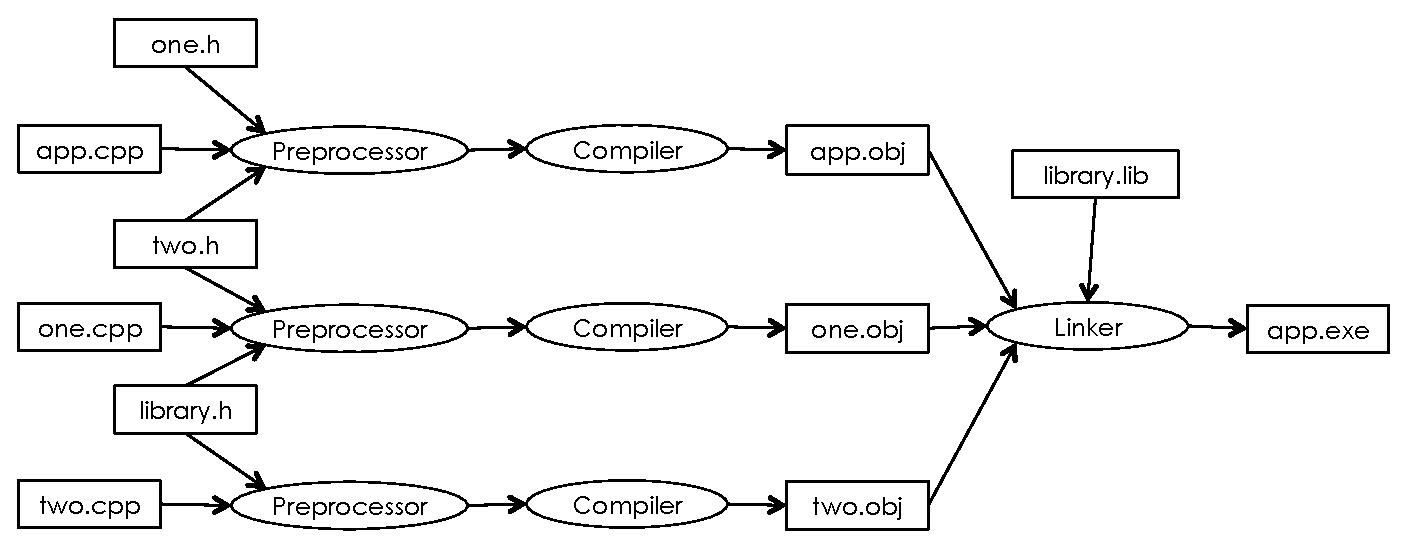
\includegraphics[width=\textwidth]{compiler_flowchart.pdf}
\end{frame}

\begin{frame}[fragile]{Modular design revisited}
    \begin{itemize}
        \item Your code can call any function for which there is a \textbf{declaration} in the current file
            (in the file itself or \lstinline{#include}d) \pause
        \item The \textbf{definition} of the function may be in another file \pause
        \item The \textbf{linker} resolves the function call in this case
    \end{itemize}
\end{frame}

\begin{frame}[fragile]{Incremental compilation}
    \begin{itemize}
        \item Compilation takes time --- compiling a AAA game can take several hours \pause
        \item Visual C++ stores intermediate files (e.g.\ \texttt{.obj} files) on disk \pause
        \item Only the changed files need to be run through the preprocessor and compiler again
            $\implies$ faster re-compilation during development \pause
        \item \textbf{Build $\to$ Clean} removes all intermediate files \pause
        \item \textbf{Build $\to$ Rebuild} forces Visual C++ to recompile everything
    \end{itemize}
\end{frame}

\begin{frame}[fragile]{Precompiled headers}
    \begin{itemize}
        \item Headers may need to be compiled multiple times if they are included in multiple source files \pause
        \item Headers may be very large ---
            e.g.\ \texttt{Windows.h} includes dozens of headers totalling many thousands of lines \pause
        \item In Visual C++ projects, \texttt{stdafx.h} is a \textbf{precompiled header} \pause
        \item \lstinline{#include "stdafx.h"} doesn't work like copy and paste ---
            instead, the compiler uses the precompiled header information \pause
        \item Precompiled header only needs to be recompiled if \texttt{stdafx.h} (or something it includes)
            changes, which should be rare
    \end{itemize}
\end{frame}

\begin{frame}[fragile]{Build configuration in VC++}
    \begin{center}
        
\includegraphics[width=0.6\textwidth]{vcpp_build_toolbar.PNG}
    \end{center}
     \pause
    \begin{itemize}
        \item Configuration:
        \begin{itemize}
            \item \textbf{Debug} allows use of the Visual C++ debugger \pause
            \item \textbf{Release} produces optimised code --- usually 2--10 $\times$ faster than Debug \pause
            \item Generally use Debug for development, Release for optimisation and distributing the finished application \pause
        \end{itemize}
        \item Platform:
        \begin{itemize}
            \item \textbf{x86} runs on 32-bit and 64-bit versions of Windows \pause
            \item \textbf{x64} runs on 64-bit Windows only \pause
            \item Generally use x86 for maximum compatibility, x64 for apps which need to use $>2$GB memory
                or where a significant speed benefit is measured
        \end{itemize}
    \end{itemize}
\end{frame}

\part{Arrays and pointers}
\frame{\partpage}

\begin{frame}[fragile]{Arrays in C++}
    \begin{itemize}
        \item An \textbf{array} is a fixed-length sequence of elements of a particular type
        \item Not to be confused with a \textbf{vector}, which is a variable length sequence
    \end{itemize}
    \begin{lstlisting}
// Declare a 5-element array with initial values
int myArray[] = { 1, 3, 5, 7, 9 };

// Declare a 10-element array without specifying initial values
int myOtherArray[10];
    \end{lstlisting}
\end{frame}

\begin{frame}[fragile]{Arrays in memory}
    \begin{center}
        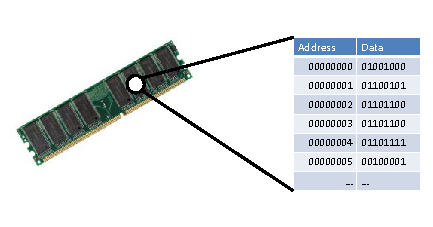
\includegraphics[width=0.6\textwidth]{memory.pdf}
    \end{center}
    \begin{itemize}
        \item An array is a contiguous block of memory
        \item E.g.\ an \lstinline{int} is 4 bytes (32 bits), so an array of 10 \lstinline{int}s is $10 \times 4 = 40$ bytes
        \item The size of the array is \textbf{fixed}: a 10 element array holds exactly 10 elements, forever
    \end{itemize}
\end{frame}

\begin{frame}[fragile]{Index out of range}
    This Python code will give a ``list index out of range'' exception
    \begin{lstlisting}[language=Python]
myList = [1, 3, 5, 7, 9]
print myList[5]
    \end{lstlisting}
    
    This C++ code will give a ``vector subscript out of range'' exception
    \begin{lstlisting}
std::vector<int> myVector = {1, 3, 5, 7, 9};
std::cout << myVector[5] << std::endl;
    \end{lstlisting}
    
    This C++ code will print some arbitrary number
    \begin{lstlisting}
int myArray[] = { 1, 3, 5, 7, 9 };
std::cout << myArray[5] << std::endl;
    \end{lstlisting}
\end{frame}

\begin{frame}[fragile]{Index out of range}
    \begin{itemize}
        \item C++ does not check array indices
        \item It is easy to accidentally read or write past the end of the array, and doing so will cause
            hard-to-fix bugs
        \item \lstinline{myArray} is a 5-element array of \lstinline{int}s, i.e.\ a block of $5 \times 4 = 20$ bytes
        \item If \lstinline{myArray} starts at memory address $1000$, then \lstinline{myArray[i]} is at address
            $1000 + 4 \times i$
        \item \lstinline{myArray[5]} is whatever happens to be at memory address $1000 + 4 \times 5 = 1020$ ---
            could be unallocated memory, could be another variable, could be part of another array,
            could even be part of the machine code being executed
    \end{itemize}
\end{frame}

\begin{frame}[fragile]{Array size must be a compile-time constant}
    \begin{lstlisting}
double a[10];            // OK

const int size = 10;
double b[size];          // OK
double c[2 * size + 7];  // OK

int varSize = 10;
double d[varSize];       // Error
    \end{lstlisting}
\end{frame}

\begin{frame}[fragile]{Dynamic allocation}
    \begin{itemize}
        \item If the size of the array is not known in advance, it can be allocated at runtime
            using the \lstinline{new} keyword
    \end{itemize}
    \begin{lstlisting}
int n = readNumberFromConsole();
int* myArray = new int[n];
    \end{lstlisting}
    \begin{itemize}
        \item Technically \lstinline{myArray} is no longer an array, it's a \textbf{pointer}
        \item \lstinline{int*} is the type ``pointer to an \lstinline{int}''
        \item Pointers can (mostly) be used as if they were arrays
    \end{itemize}
\end{frame}

\begin{frame}[fragile]{Stack and heap}
    \begin{itemize}
        \item Variables and static arrays are stored on the \textbf{stack}
        \begin{itemize}
            \item Stack items are automatically freed when they go out of scope
        \end{itemize}
        \item Anything created with \lstinline{new} is stored on the \textbf{heap}
        \begin{itemize}
            \item Heap items must be freed with \lstinline{delete} when they are finished with
            \item Forgetting to free them is a \textbf{memory leak}
        \end{itemize}
    \end{itemize}
\end{frame}

\begin{frame}[fragile]{Strings revisited}
    \begin{itemize}
        \item \lstinline{std::string} is the high-level string class
        \item The low-level way of storing strings is as an array of \lstinline{char}s
    \end{itemize}
    \begin{lstlisting}
char greeting[] = "Hello, world!";
    \end{lstlisting}
    \begin{itemize}
        \item Strings are \textbf{null terminated} --- they end with ASCII character 0
    \end{itemize}
\end{frame}

\begin{frame}[fragile]{String literals}
    \begin{lstlisting}
std::string greeting = "Hello, world!";
    \end{lstlisting}
    \begin{itemize}
        \item The thing on the right hand side is actually a \lstinline{char} array, not a \lstinline{std::string}
        \item The assignment operator knows how to convert from \lstinline{char[]} to \lstinline{std::string}
    \end{itemize}
\end{frame}

%\begin{frame}[fragile]{Pointers}
%    \begin{itemize}
%        \item C++ allows us to store and manipulate \textbf{pointers} a.k.a.\ memory addresses
%    \end{itemize}
%    \begin{lstlisting}
%int myVar = 7;
%int* myPointer = &myVar;
%*myPointer = 12;
%    \end{lstlisting}
%    \begin{itemize}
%        \item \lstinline{int*} is a type: pointer to int
%        \item \lstinline{&} is the \textbf{address-of} operator:
%            read \lstinline{&myVar} as ``a pointer to \lstinline{myVar}''
%        \item \lstinline{*} on line 3 is the \textbf{dereference} operator:
%            read \lstinline{*myPointer} as ``the value pointed to by \lstinline{myPointer}''
%    \end{itemize}
%\end{frame}

\begin{frame}[fragile]{2-dimensional arrays}
    Array of arrays approach:
    \begin{lstlisting}
const int width = 8, height = 8;
int grid[width][height];
grid[x][y] = 7;
    \end{lstlisting}
    Flat array approach:
    \begin{lstlisting}
const int width = 8, height = 8;
int grid[width * height];
grid[x + y * width] = 7;
    \end{lstlisting}
\end{frame}


\part{Functions}
\frame{\partpage}

\begin{frame}[fragile]{Function definitions}
    \begin{itemize}
        \item We have already seen an example of a function definition
    \end{itemize}
    \begin{lstlisting}
int main()
{
    std::cout << "Hello, world!" << std::endl;
    return 0;
}
    \end{lstlisting}
    \begin{itemize}
        \item The function \lstinline{main} takes no parameters, and returns a value of type \lstinline{int}
    \end{itemize}
\end{frame}

\begin{frame}[fragile]{Function signatures}
    \begin{itemize}
        \item The \textbf{signature} of a function defines its return type, name, and parameters
    \end{itemize}
    \begin{lstlisting}
double foo(std::string x, int y, bool z)
    \end{lstlisting}
    \pause
    \begin{itemize}
        \item This function takes three parameters: \pause
        \lstinline{x} of type \lstinline{std::string}, \pause
        \lstinline{y} of type \lstinline{int}, \pause
        and \lstinline{z} of type \lstinline{bool} \pause
        \item It returns a value of type \lstinline{double}
    \end{itemize}
\end{frame}

\begin{frame}[fragile]{Functions without return values}
    \begin{itemize}
        \item It is possible to define a function which does not return a value, using the \lstinline{void} keyword
        in place of its return type
    \end{itemize}
    \pause
    \begin{lstlisting}
void printNumber(int n)
{
    std::cout << n << std::endl;
}
    \end{lstlisting}
\end{frame}

\begin{frame}[fragile]{Pass by value}
    \begin{itemize}
        \item Function parameters are passed \textbf{by value}:
        the function receives \textbf{copies} of the original variables
    \end{itemize}
    \pause
    \begin{lstlisting}
void changeName(std::string name)
{
    name = "Ed";
}

int main()
{
    std::string name = "Mike";
    std::cout << name << std::endl; // Mike
    changeName();
    std::cout << name << std::endl; // Mike
}
    \end{lstlisting}
\end{frame}

\begin{frame}[fragile]{Pass by reference}
    \begin{itemize}
        \item Parameters can be passed \textbf{by reference} using \lstinline{&}, allowing the function to modify them
    \end{itemize}
    \pause
    \begin{lstlisting}
void changeName(std::string& name)
{
    name = "Ed";
}

int main()
{
    std::string name = "Mike";
    std::cout << name << std::endl; // Mike
    changeName();
    std::cout << name << std::endl; // Ed
}
    \end{lstlisting}
\end{frame}

\begin{frame}[fragile]{One area where C++ is ``simpler'' than Python!}
    \begin{itemize}
        \item Recall from COMP110 week 6: in Python, basic data types (numbers, booleans, strings etc)
            are passed by value, and object types (lists, dictionaries, class instances) are passed by reference
        \pause
        \item In C++, everything is passed by value unless it is explicitly marked as a reference with \lstinline{&}
    \end{itemize}
\end{frame}

\begin{frame}[fragile]{Constant references}
    \begin{lstlisting}
void greet(std::string name)
{
    std::cout << "Hi " << name << std::endl;
}
    \end{lstlisting}
    \pause
    \begin{itemize}
        \item The string will be copied in order to be passed in \pause
        \item More efficient to pass a reference, and mark it \lstinline{const} to prevent accidental modification
    \end{itemize}
    \begin{lstlisting}
void greet(const std::string& name)
{
    std::cout << "Hi " << name << std::endl;
}
    \end{lstlisting}
    \pause
    \begin{itemize}
        \item (this is only worthwhile for large data structures like strings and vectors, not for basic data types)
    \end{itemize}
\end{frame}



\part{Live coding: Noughts and Crosses}
\frame{\partpage}

% -------------------------------------------------------

%\part{The compiler}
%\frame{\partpage}
%
%\begin{frame}
%	\frametitle{The build process}
%	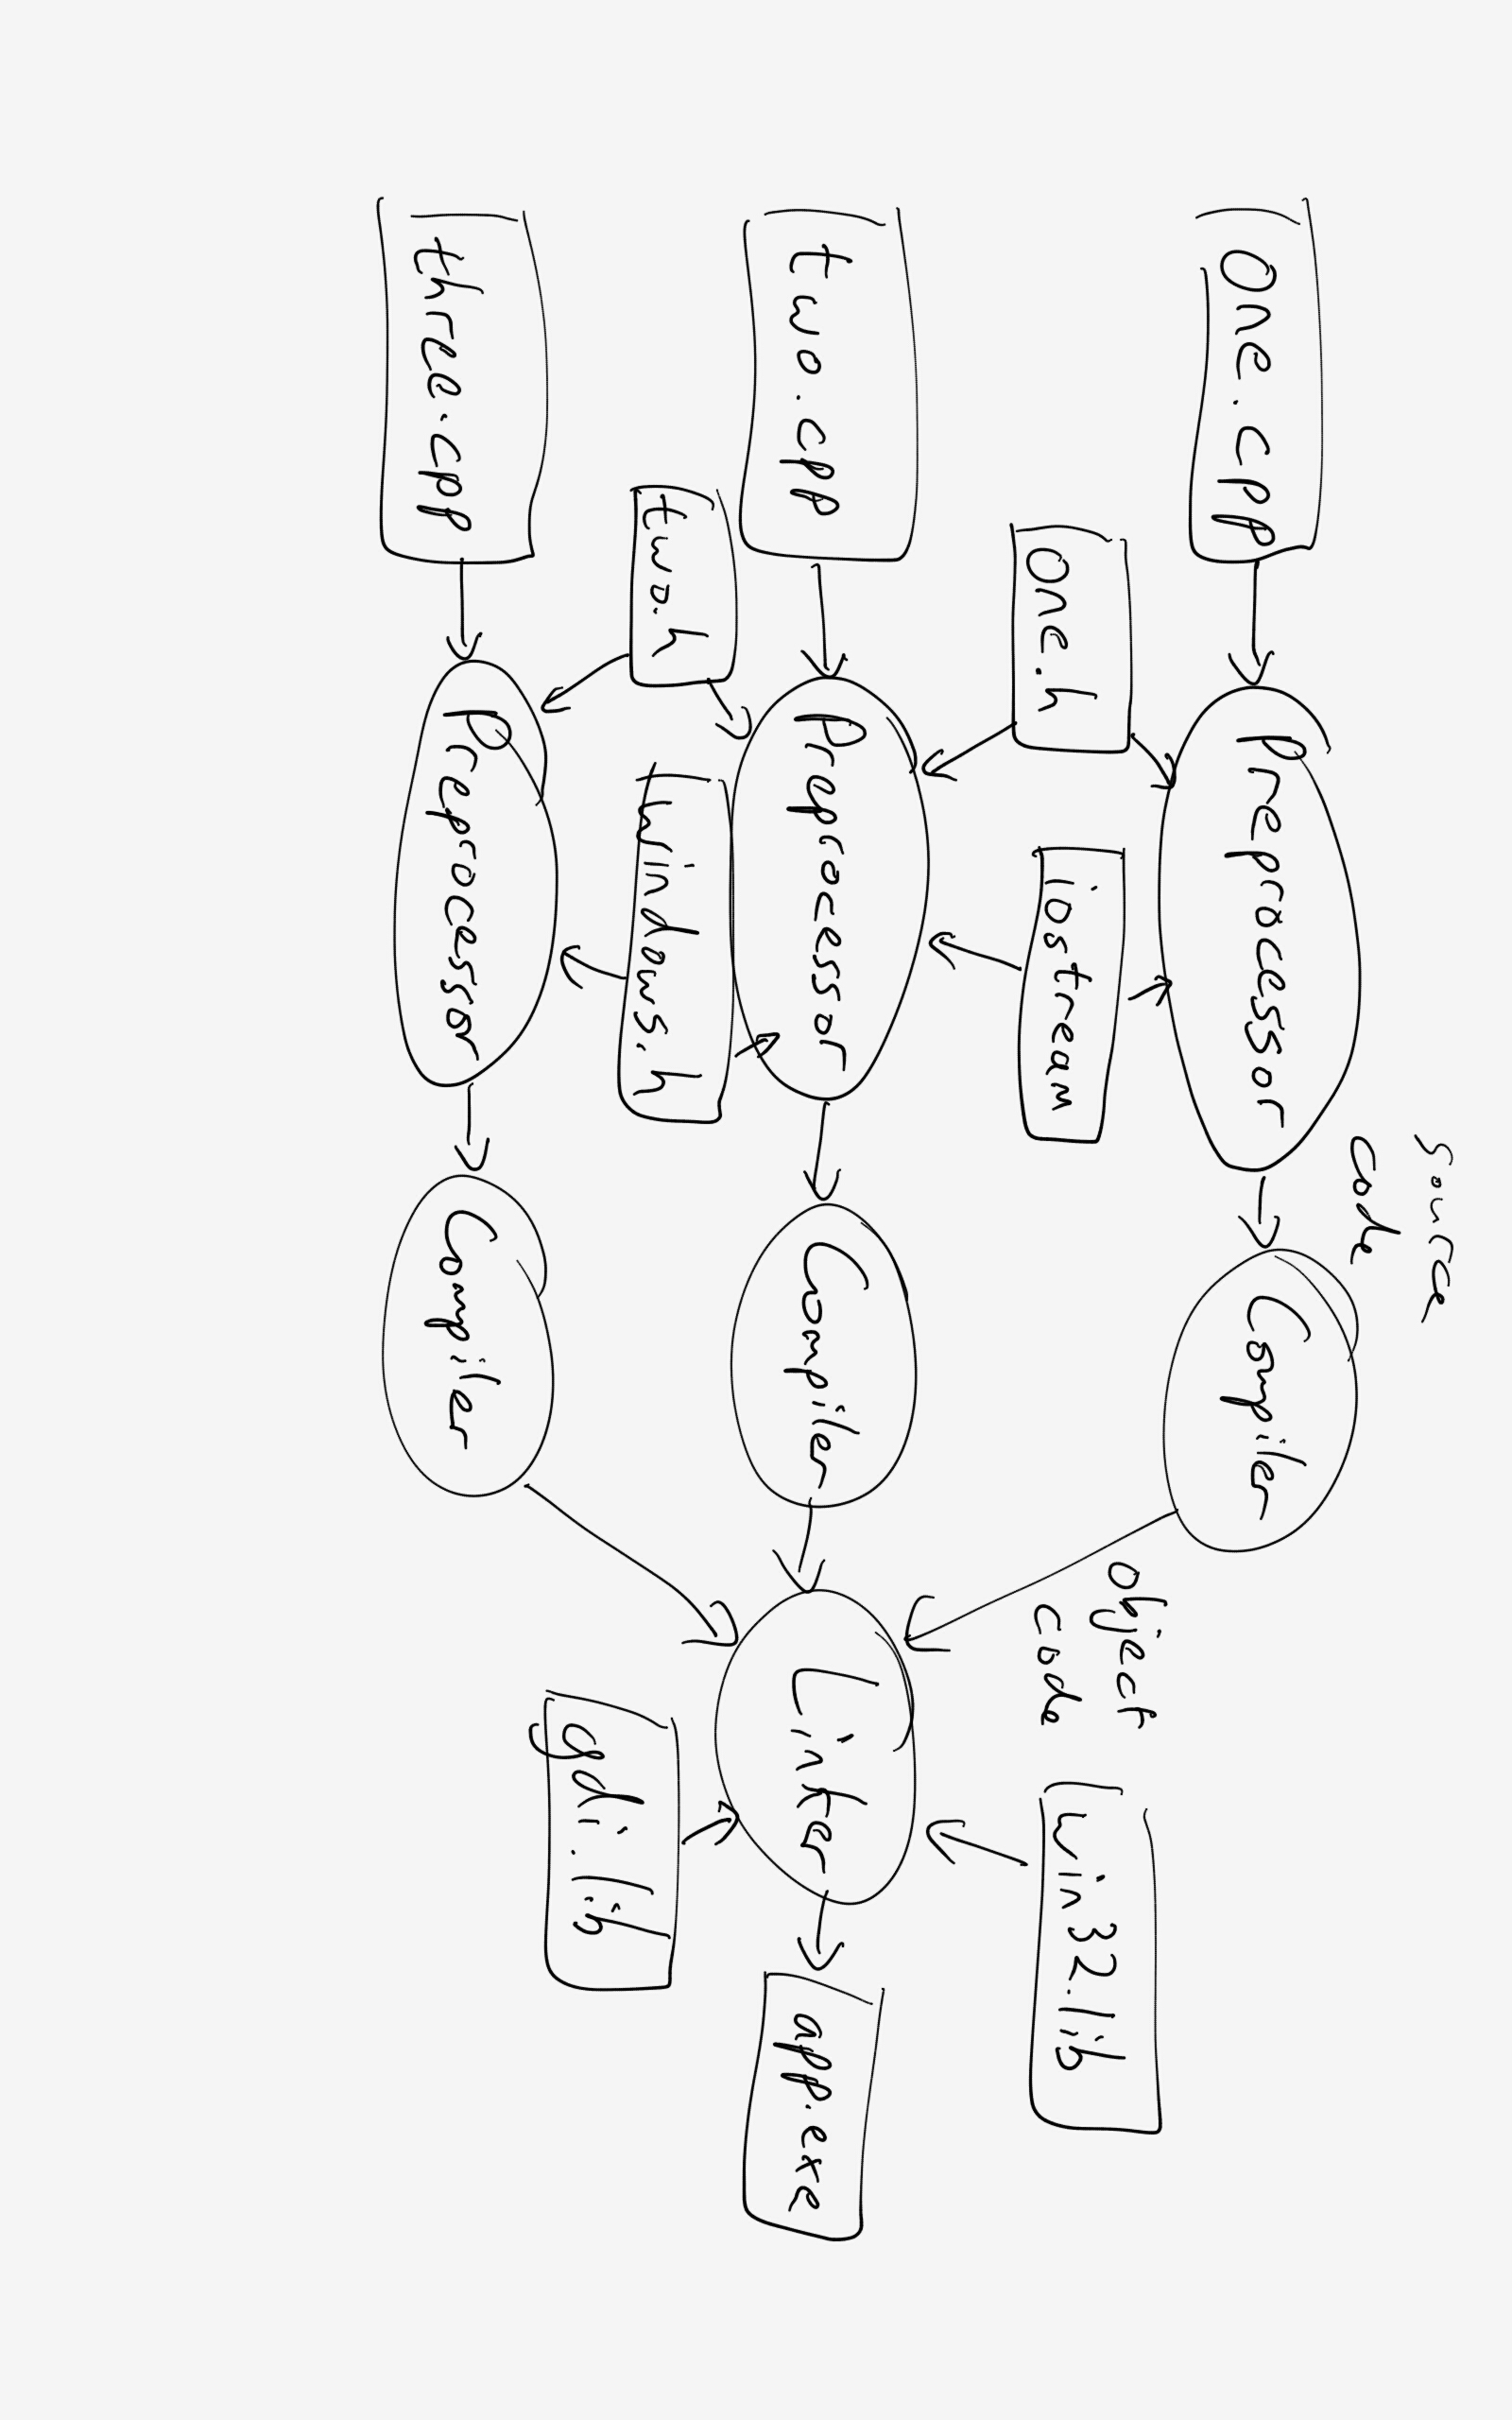
\includegraphics[height=\textwidth,angle=90]{compiler_sketch}
%\end{frame}

\end{document}
